% =============================================================================
%  Breadcrumbs
%  Blockchain Olympiad submission, Team CookieMonsters, United International
%  University.
%
%  HOW TO COMPILE
%    Upload main.tex and ref.bib to Overleaf. Set the compiler to pdfLaTeX.
%    Overleaf runs BibTeX automatically. Nothing else is needed: every figure
%    is drawn in TikZ inside this file, so there are no image files to upload.
%
%  >>> EDIT THE TEAM BLOCK BELOW BEFORE SUBMITTING <<<
% =============================================================================
\documentclass[11pt,border=6pt,varwidth=20cm]{standalone}

% ---- team details: replace the bracketed placeholders -----------------------
\newcommand{\TeamName}{CookieMonsters}
\newcommand{\TeamInstitution}{United International University, Dhaka, Bangladesh}
\newcommand{\TeamMembers}{Ahbab, Ruhi, Rohan, Ishmam, Adnan}
\newcommand{\TeamCategory}{Undergraduate}
\newcommand{\TeamContact}{mkhan223869@bscse.uiu.ac.bd}
% -----------------------------------------------------------------------------

\usepackage[T1]{fontenc}
\usepackage[utf8]{inputenc}
\usepackage{lmodern}

\usepackage{amsmath,amssymb}
\usepackage{graphicx}
\usepackage{xcolor}
\usepackage{booktabs}
\usepackage{tabularx}
\usepackage{array}
\usepackage{longtable}
\usepackage{caption}
\usepackage{enumitem}
\usepackage{titlesec}

\usepackage{tikz}
\usepackage{pgfplots}
\usepackage{algorithm}
\usepackage{algpseudocode}



\usetikzlibrary{positioning,shapes.geometric,arrows.meta,calc,fit,backgrounds}
\pgfplotsset{compat=1.18}

% ---- palette (colour-blind safe, prints correctly in greyscale) -------------
\definecolor{tcblue}{HTML}{2563EB}
\definecolor{tcorange}{HTML}{E8710A}
\definecolor{tcgreen}{HTML}{059669}
\definecolor{tcgrey}{HTML}{6B7280}
\definecolor{tctext}{HTML}{111827}
\definecolor{tcline}{HTML}{E5E7EB}
\definecolor{tcbg}{HTML}{F7F8FA}


\captionsetup{font=small,labelfont={bf,sf}}
\setlength{\parskip}{0.35em}
\renewcommand{\arraystretch}{1.18}




\newcolumntype{Y}{>{\raggedright\arraybackslash}X}
\newcommand{\est}{\textsuperscript{\textdagger}}

% ---- the logo, drawn rather than imported ----------------------------------
% A trail of marks, each one larger and more definite than the last, ending in
% the verified record. Drawn rather than imported so the file stays standalone.
\newcommand{\bclogo}[1][1.0]{%
\begin{tikzpicture}[scale=#1,every node/.style={transform shape}]
  \node[regular polygon,regular polygon sides=6,draw=tcblue,line width=1.5pt,
        minimum size=2.35cm,rotate=90] (hex) at (0,0) {};
  \draw[tcgrey!45,line width=1.0pt,dash pattern=on 1pt off 2.6pt,line cap=round]
        (-0.53,-0.36) -- (0.53,0.36);
  \fill[tcgrey!55] (-0.53,-0.36) circle (0.085);
  \fill[tcgrey]    (-0.27,-0.17) circle (0.110);
  \fill[tcblue]    ( 0.00, 0.00) circle (0.135);
  \fill[tcorange]  ( 0.27, 0.17) circle (0.155);
  \fill[tcgreen]   ( 0.53, 0.36) circle (0.180);
\end{tikzpicture}}

\begin{document}
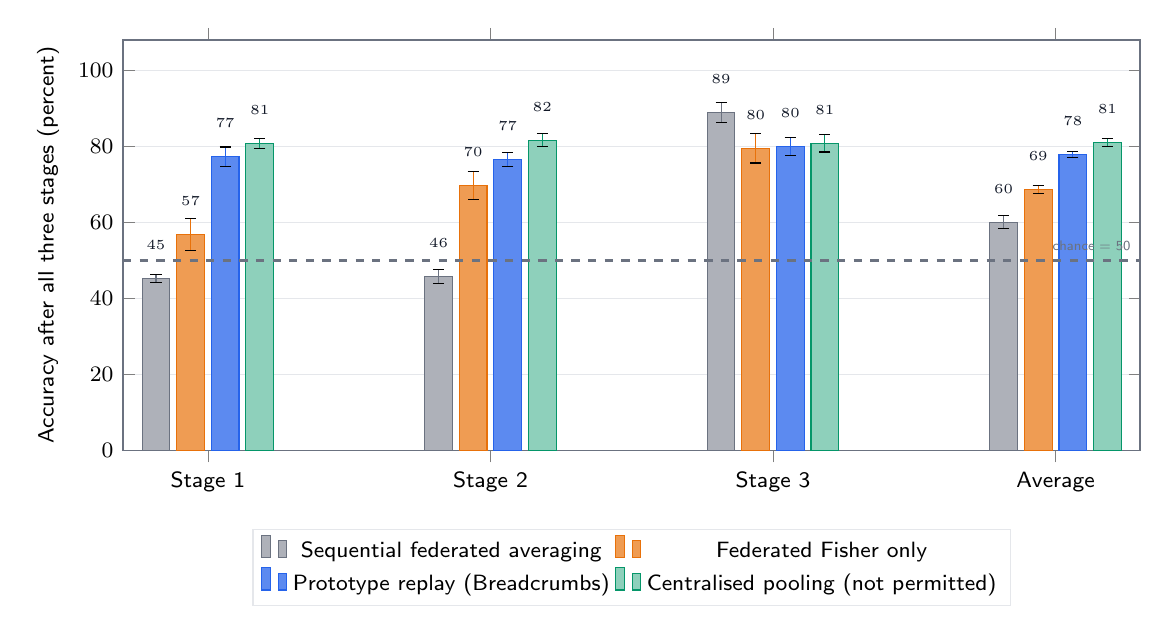
\begin{tikzpicture}
\begin{axis}[
  width=14.5cm, height=6.8cm,
  ybar=2.5pt, bar width=10pt,
  font=\sffamily\small,
  ymin=0, ymax=108, ytick={0,20,40,60,80,100},
  ylabel={Accuracy after all three stages (percent)},
  symbolic x coords={Stage 1, Stage 2, Stage 3, Average},
  xtick=data,
  ymajorgrids=true, grid style={tcline,line width=0.5pt},
  axis line style={tcgrey,line width=0.6pt},
  tick label style={font=\sffamily\footnotesize},
  label style={font=\sffamily\footnotesize},
  legend style={font=\sffamily\footnotesize,at={(0.5,-0.19)},anchor=north,
                legend columns=2,draw=tcline},
  nodes near coords, every node near coord/.append style={
      font=\sffamily\tiny,color=tctext,yshift=7pt,
      /pgf/number format/fixed,/pgf/number format/precision=0},
  error bars/y dir=both, error bars/y explicit,
]
\addplot[fill=tcgrey!55,draw=tcgrey] coordinates {
  (Stage 1,45.2) +- (0,1.1) (Stage 2,45.8) +- (0,1.8)
  (Stage 3,88.9) +- (0,2.7) (Average,60.0) +- (0,1.7)};
\addplot[fill=tcorange!70,draw=tcorange] coordinates {
  (Stage 1,56.8) +- (0,4.3) (Stage 2,69.6) +- (0,3.7)
  (Stage 3,79.5) +- (0,3.9) (Average,68.6) +- (0,1.1)};
\addplot[fill=tcblue!75,draw=tcblue] coordinates {
  (Stage 1,77.3) +- (0,2.5) (Stage 2,76.5) +- (0,1.8)
  (Stage 3,79.9) +- (0,2.3) (Average,77.9) +- (0,0.8)};
\addplot[fill=tcgreen!45,draw=tcgreen] coordinates {
  (Stage 1,80.7) +- (0,1.3) (Stage 2,81.6) +- (0,1.7)
  (Stage 3,80.8) +- (0,2.3) (Average,81.0) +- (0,1.0)};
\draw[tcgrey,dashed,line width=0.9pt]
  ({rel axis cs:0,0}|-{axis cs:Stage 1,50}) -- ({rel axis cs:1,0}|-{axis cs:Stage 1,50});
\node[font=\sffamily\tiny,text=tcgrey,anchor=south east]
  at ({rel axis cs:1,0}|-{axis cs:Stage 1,50}) {chance = 50};
\legend{Sequential federated averaging, Federated Fisher only,
        Prototype replay (Breadcrumbs), Centralised pooling (not permitted)}
\end{axis}
\end{tikzpicture}
\end{document}
